\input{./._relpath-to-latexroot.ltx}
\documentclass[\latexroot/\projectname]{subfiles}
\input{\latexroot/@resources/subfile-setup.ltx}
\begin{document}
\whenstandalone{%
  \graphicspath{{../images/}}%
}%
\whenintegrated{%
  \graphicspath{{./images/}}%
}%

\FloatBarrier
\section{Inspecting the Model's Mechanisms}
\whenintegrated{\label{sec:hank}}

Recent literature has cast doubt on the relevance of borrowing constraints to entrepreneurial entry \citep{Hurst2004-sf} and on the size of the returns to entrepreneurship \citep{Moskowitz2002-ax}. High wealth inequality in our model is generated by the combination of occupational choice in the presence of borrowing constraints and high potential returns to entrepreneurship. We check here whether the observable implications generated by our model are consistent with the observed data.

\subsection{Borrowing Constraints and Entry}

The main finding of \cite{Hurst2004-sf} is that the probability of entering entrepreneurship is almost flat over a large portion of the wealth distribution and then increases for the richest workers. There are two main points worth discussing.

First, the results of our paper do not depend in important ways on the fact that the financial constraint affects the decision to become an entrepreneur. Rather, it is the greater incentive to save after entry that is crucial for the results.

Second, our model of occupational choice with borrowing constraints produces entry decisions that are consistent with the Hurst--Lusardi finding. We generate many samples of households from our model and estimate a probit regression of entry probability as a function of wealth.

\begin{figure}[htbp]
  \centering
  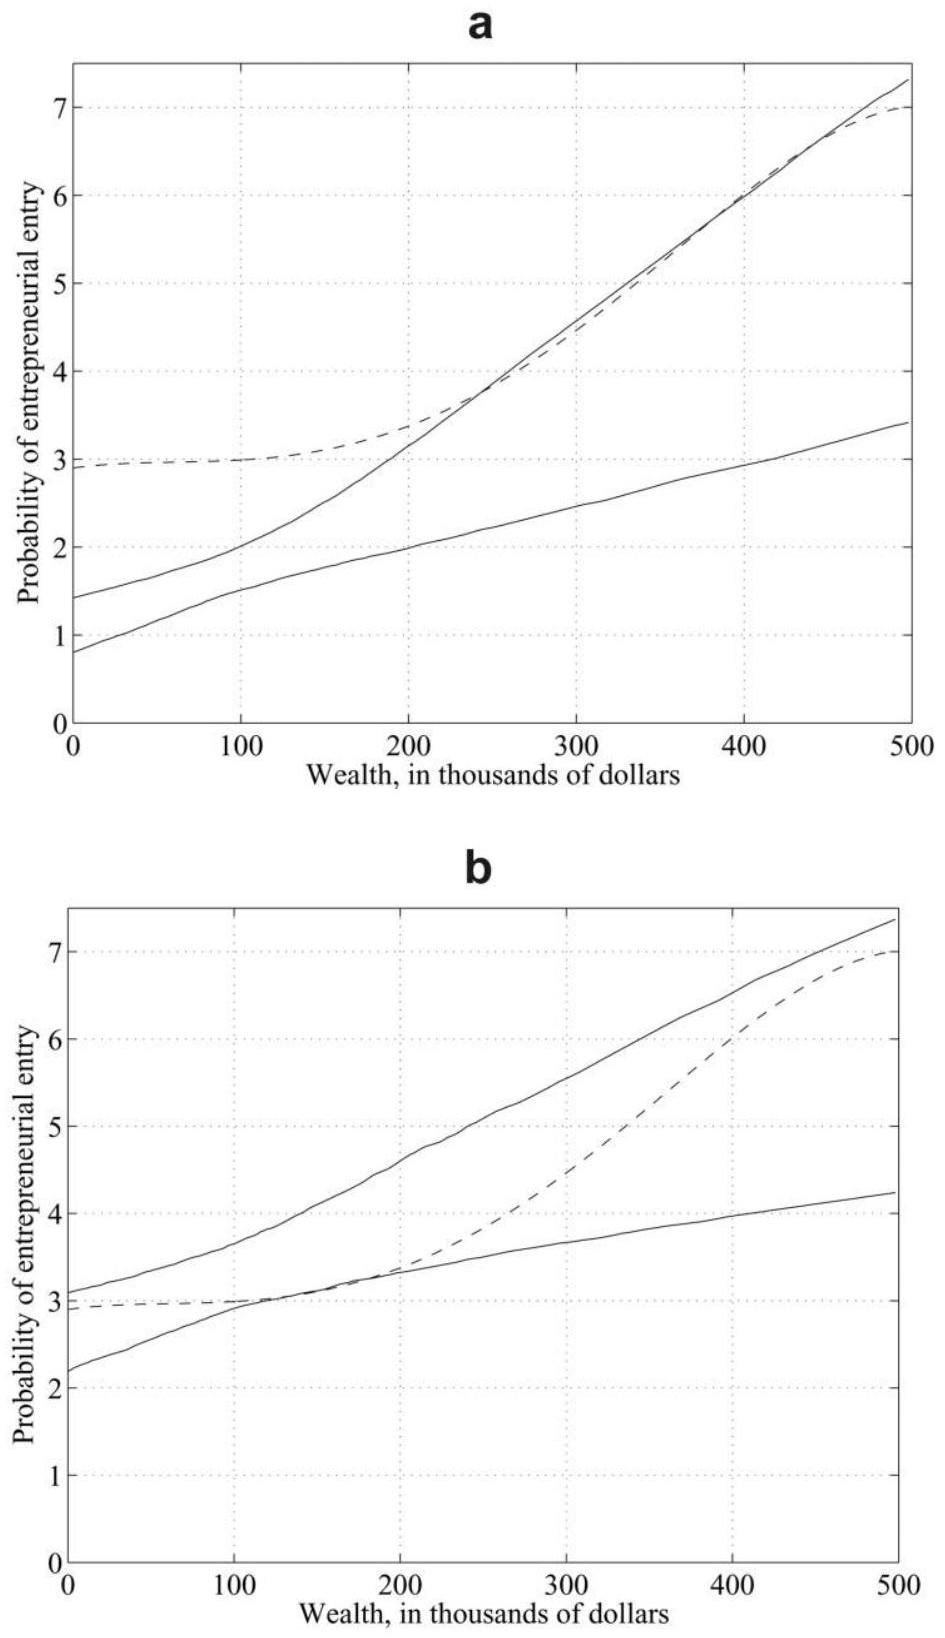
\includegraphics[width=0.85\textwidth]{entry_probability.jpg}
  \caption{Probability of entering entrepreneurship as a function of own wealth as estimated by Hurst and Lusardi (dashed line), and confidence interval generated by two versions of the model (solid lines). $a$, Benchmark model. $b$, Benchmark with a small fraction of nonentrepreneurial self-employed.}
  \whenintegrated{\label{fig:entry-probability}}
\end{figure}

Both Hurst and Lusardi's estimates and our confidence intervals are consistent with an entry probability that is a convex function of wealth. In the presence of borrowing constraints, a worker with high entrepreneurial ability is likely to save to enter entrepreneurship. As a result, we are not very likely to observe many high-ability potential entrepreneurs among the poor. Given only one type of entrepreneurial ability and that none of the calibrated parameters were chosen to match this aspect of the data, it is remarkable how our model is not inconsistent with flat entry probabilities over large sections of wealth holdings.

\subsection{Returns from Private Business Ownership}

\cite{Moskowitz2002-ax} cast doubt on the assumption that entrepreneurs face potentially high rates of return. We compare the cross-sectional distribution of returns to entrepreneurship in our model and in the data using the 1989 SCF wave.

\begin{table}[htbp]
  \centering
  \caption{Distribution of Rates of Return (\%) for Self-Employed Business Owners}
  \whenintegrated{\label{tab:returns}}
  \begin{tabular}{lcccc}
    \hline\hline
    & \multicolumn{4}{c}{Percentile} \\
    \cline{2-5}
    & 25th & 50th & 75th & 90th \\
    \hline
    Only income from business & 0 & 3 & 25 & 143 \\
    Including wages and salaries & 10 & 40 & 125 & 520 \\
    \hline
  \end{tabular}
\end{table}

The size of the returns to private equity crucially hinges on how income from the firm is divided between entrepreneurial wages and return to capital. The median distribution of returns is 49 percent in our model compared to 40 percent in the data, so our median entrepreneurial return is only a little higher in our model than in the SCF data.

\smartbib

\end{document}
